% =====================================================================
%  AURA preparatory report -- main file
%  Build: see README.md  (xelatex -> biber -> xelatex -> xelatex)
%  Shared file: change only after agreeing with your partner.
% =====================================================================
\documentclass{aura-report}
\addbibresource{references.bib}
\graphicspath{{figures/}}

\reporttitle{השקת \en{AURA}:\\ מותג טינט שפתיים בהשראת מזון}
            {Launching AURA: A Food-Inspired Lip Tint Brand}
\reportsubtitle{תוכנית השקה, חקר שוק וניהול סיכונים}
\course{יישומי \en{Vibe Coding} ו-\en{AI} במדע וביום-יום}{AI Agents \& Vibe Coding}
\institution{אוניברסיטת חיפה}{University of Haifa}
\lecturer{ד"ר יורם סגל}{Dr. Yoram Segal}
\addauthor{Raneem Daher}{רנים דאהר}
\addauthor{Raghad Rabah}{רגאד רבאח}
\copyrightholder{Raneem Daher \& Raghad Rabah}

\begin{document}

\makecover

% ----- Front matter (pages numbered with Hebrew letters) -----
\frontmatter
% =====================================================================
%  Front matter: executive summary + keywords
%  Booklet: 250-350 words, one continuous block. Written LAST.
%  Owner: shared (front matter)
% =====================================================================
\chapter*{תקציר מנהלים}
\addcontentsline{toc}{chapter}{תקציר מנהלים}
\markboth{תקציר מנהלים}{}

דוח מכין זה מציג תוכנית השקה בת \ltr{6} חודשים בישראל עבור \en{AURA}, מותג
טינט שפתיים בהשראת מזון, לנשים בנות \ltr{18--28}. הרקע הוא שתי מגמות עולמיות:
מוצרי השפתיים הפכו למנוע צמיחה באיפור, ומוצרי יופי מתגלים יותר ויותר ברשתות
החברתיות. שוק הקוסמטיקה בישראל מוערך ב-\ltr{\$408.53} מיליון בשנת \ltr{2026},
וקהל היעד המיידי כולל כ-\ltr{211} אלף סטודנטיות. הבעיה היא שמותג חדש מתחיל
מאפס מודעות, בשוק שבו מתחרי הפרימיום עולים \ltr{99--175} ש"ח ונרכשים מרחוק,
ומוצר שנבחר לפי גוון, מרקם וניחוח קשה למכור בלי התנסות. לכן הוגדרו חמישה יעדי
\en{SMART}, ובהם מודעות של \ltr{20\%} לפחות בקמפוסי הפיילוט ומכירות של \ltr{255}
אלף ש"ח בחודשים \ltr{4--6}, ומפרט של \ltr{11} דרישות עם ערכי יעד ושיטות אימות.
סקירת \ltr{12} מאמרים שפיטים מראה שגירויים חושיים, שמות מפתיעים, משפיענים
אמינים ודוגמיות חינם אפקטיביים כל אחד בנפרד, אך שילובם בהשקה של מותג קוסמטיקה
לא נבדק; מאמר הדגל מספק מודל למדידת השפעת הדוגמיות דרך הרחבה, האצה
וקניבליזציה, וההשקה תמדוד בהתאם כמה מהקונות בדוכנים הן קונות חדשות באמת. חקר
השוק מזהה חלל \en{Masstige} סביב מחיר של \ltr{69} ש"ח, בין מוצרי הפארם הזולים
לבין מותגי הפרימיום המיובאים, ומעריך את השוק הזמין בפלח הסטודנטיות בכ-\ltr{25.55}
מיליון ש"ח בשנה; יעד ההשקה הוא נתח קטן ושמרני ממנו. מבין שלוש חלופות, נבחרה
במטריצת החלטה משוקללת החלופה ההיברידית (ציון \ltr{8.10}, לעומת \ltr{7.40}
ו-\ltr{6.45}): אתר \en{D2C}, מרקטפלייס ישראלי, \ltr{20--30} משפיעניות קטנות
ושלושה ברי טעימות בקמפוסים, שבהם הקונות טועמות את המזון ומנסות את הגוון.
תוכנית העבודה מחלקת את ההשקה לשש חבילות עבודה ושש אבני דרך בתקציב של \ltr{150}
אלף ש"ח, עם שער \en{Go/No-Go} בסוף החודש השלישי, שבו נבדקות הודעות השיווק
למשרד הבריאות. ניתוח הסיכונים מזהה שבעה סיכונים, ותוכנית ההפחתה מורידה את
החשיפה המרבית מציון \ltr{16} ל-\ltr{6}. המסקנה: התוכנית מוכנה לביצוע, והצעד
הראשון הוא הגשת ההודעות למשרד הבריאות.

\keywords{השקת מותג \sep ביוטי בהשראת מזון \sep שיווק משפיענים \sep דוגמיות \sep שיווק חושי \sep אומניצ'אנל}

\tableofcontents
\listoffigures
\listoftables
% =====================================================================
%  Front matter: list of abbreviations and terms (alphabetical)
%  Owner: shared - each partner adds the terms of her own chapters.
% =====================================================================
\chapter*{רשימת קיצורים ומונחים}
\addcontentsline{toc}{chapter}{רשימת קיצורים ומונחים}
\markboth{רשימת קיצורים ומונחים}{}

\begin{abbreviations}
\abbr{CAGR}{שיעור צמיחה שנתי ממוצע (\en{Compound Annual Growth Rate})}
\abbr{RACI}{מטריצת אחריות: מבצע, אחראי, מיועץ, מיודע}
\abbr{SAM}{השוק הזמין לשירות (\en{Serviceable Available Market})}
\abbr{SOM}{נתח השוק הניתן להשגה (\en{Serviceable Obtainable Market})}
\abbr{TAM}{השוק הכולל (\en{Total Addressable Market})}
\abbr{WBS}{מבנה פירוק העבודה (\en{Work Breakdown Structure})}
\end{abbreviations}


% ----- Body (pages 1-40) -----
\mainmatter
% =====================================================================
%  Chapter 1: Introduction and background        Page budget: 3 (pp. 1-3)
%  Booklet (ch. 3): a funnel - global trends -> application context ->
%           motivation (why existing approaches are not enough) ->
%           structure of the report.
%  Owner: Raneem (Claude Code) - only she edits this file
% =====================================================================
\chapter{מבוא ורקע}
\label{ch:intro}

דוח זה מציג תוכנית השקה בת \ltr{6} חודשים בישראל עבור \en{AURA}, מותג טינט
שפתיים בהשראת מזון שפותח בתרגיל \ltr{1}. קהל היעד הוא נשים בנות \ltr{18--28},
וערוצי ההשקה הם \en{TikTok} ו-\en{Instagram}, משפיעניות קטנות
(\en{Micro-Influencers}) ודוכני טעימות בקמפוסים. המבוא בנוי כמשפך: הוא פותח
בשלוש מגמות עולמיות, עובר להקשר הישראלי, מסביר מדוע דרכי ההשקה המקובלות אינן
מספיקות למותג חדש, ומסתיים במפת הדוח.

\section{מגמות עולמיות: ביוטי בהשראת מזון ומסחר חברתי}
\label{sec:intro-trends}

\textbf{ביוטי בהשראת מזון.} קטגוריית מוצרי השפתיים היא כיום מנוע צמיחה מרכזי
באיפור: בשוק הביוטי היוקרתי בארה"ב צמחה הקטגוריה ב-\ltr{19\%} בשנת \ltr{2024},
לעומת \ltr{5\%} באיפור כולו~\cite{circana2025beauty}, ומגמה זו נמשכה
ב-\ltr{2025}~\cite{glossy2025lips}. בתוך הקטגוריה מתחזק גל המוצרים בהשראת מזון
(\en{Food-Inspired Beauty}), שעבר משלב של גימיק לקטגוריה בפני
עצמה~\cite{waldeck2026foodbased}. דוגמה בולטת היא שפתון בהשראת חמוצים של
\en{e.l.f. Cosmetics}, שאזל תוך \ltr{8} דקות; לפי החברה, \ltr{77\%} מרוכשיו
היו לקוחות חדשים של המותג~\cite{waldeck2026foodbased}. גם חיפושי ניחוח ``גויאבה''
זינקו ב-\ltr{1,000\%} בשנה אחת, לפי נתוני \en{Spate}~\cite{jensen2025guava}.
אנשי התעשייה מסבירים את המשיכה בכך שמזון מוכר ונגיש לכל אחד: שם של פרי או
קינוח מעורר תחושה ואווירה שגוון לבדו אינו מעורר~\cite{jensen2025guava,waldeck2026foodbased}.

\textbf{מסחר חברתי ודור \en{Z}.} הרשתות החברתיות הפכו לנקודת הגילוי העיקרית של
מוצרי יופי בקרב דור \en{Z}. לפי סקר של סוכנות המשפיענים \en{Kyra},
\en{TikTok} מוביל כפלטפורמת גילוי (\ltr{39\%}), ואחריו \en{Instagram}
(\ltr{35\%}); נתח הרכישות דרך מסחר חברתי (\en{Social Commerce}) הוכפל
ל-\ltr{12\%}, ודור \en{Z} נוטה לנסות מותגים חדשים יותר מאשר לשמור נאמנות
למותג קיים~\cite{meintjes2025genz}. במקביל צומח שוק שיווק המשפיענים
(\en{Influencer Marketing}) מ-\ltr{\$21.1} מיליארד בשנת \ltr{2024}
ל-\ltr{\$24} מיליארד בשנת \ltr{2025}, ורוב היוצרים ב-\en{Instagram} (\ltr{76\%})
הם משפיעני ננו עם אלפי עוקבים בלבד~\cite{hypeauditor2025state}.

\section{ההקשר הישראלי}
\label{sec:intro-israel}

שוק מוצרי הקוסמטיקה בישראל מוערך ב-\ltr{\$408.53} מיליון בשנת \ltr{2026}, וצפוי
לצמוח עד \ltr{2031} בשיעור שנתי ממוצע (\en{CAGR}) של \ltr{4.60\%}. בין מנועי
הצמיחה נמנים מגזר היוקרה הנגישה (\en{Masstige}) והמסחר
המקוון~\cite{mordor2026israel}. התשתית הדיגיטלית לפנייה ישירה לקהל קיימת: בישראל
כ-\ltr{5.00} מיליון משתמשי \en{Instagram} וכ-\ltr{4.49} מיליון משתמשי
\en{TikTok} בגיל \ltr{18} ומעלה~\cite{datareportal2026israel}. קהל היעד מרוכז גם
פיזית: בשנת הלימודים תשפ"ז צפויים ללמוד כ-\ltr{350,900} סטודנטים ב-\ltr{57}
מוסדות~\cite{che2026students}, ונשים הן \ltr{60.3\%} מהלומדים לתואר
אקדמי~\cite{cbs2024students}. כפי שמפורט בפרק~\ref{ch:market}, מדובר בכ-\ltr{211}
אלף סטודנטיות --- קהל שאפשר להגיע אליו גם ברשת וגם בקמפוס.

עם זאת, השוק המקומי צפוף ומקוטב. מותגי הטינט הוויראליים מחו"ל נרכשים בישראל בעיקר דרך
יבוא מקביל, דיוטי פרי או משלוח מחו"ל, ומחירם לצרכנית מגיע ל-\ltr{99--175}
ש"ח~\cite{rhode2026terms,makeupstore2026rhode,caretobeauty2026benefit}; בקצה השני
עומדים מוצרי פארם זולים, סביב \ltr{15} ש"ח, ללא סיפור מותג~\cite{essence2026superpharm}.
בין שני הקצוות נותר פער מחיר, ש-\en{AURA} מכוונת אליו במחיר של \ltr{69} ש"ח
(פרק~\ref{ch:market}).

\section{מוטיבציה: מדוע הגישות הקיימות אינן מספיקות}
\label{sec:intro-motivation}

הדרכים המקובלות להשקת מותג קוסמטיקה אינן מתאימות למותג חדש וקטן בשוק הזה, משלוש
סיבות:

\begin{itemize}
  \item \textbf{מדף בפארם בלבד.} מוצר שעומד על מדף, לצד מותגים מוכרים, אינו
    בונה מודעות בעצמו. מותג שאיש לא שמע עליו זקוק לסיבה להיבחר.
  \item \textbf{פרסום ממומן או סלבריטאים.} תקציב השקה מוגבל אינו מאפשר קמפיין
    רחב, ודור \en{Z} מושפע מיוצרי תוכן לפחות כמו מחברים~\cite{meintjes2025genz}.
    משפיעניות קטנות זמינות בשפע: ברשת \en{Instagram}, \ltr{76\%} מכלל
    היוצרים הם משפיעני ננו~\cite{hypeauditor2025state}.
  \item \textbf{מכירה מקוונת בלבד.} מוצר שכל ערכו בגוון, במרקם ובניחוח קשה למכור
    מבלי לנסות אותו. בסקר של \ltr{20,000} צרכנים, \ltr{75\%} השיבו כי סביר
    יותר שירכשו ממותג שלא הכירו לאחר שקיבלו דוגמית, ורק \ltr{33\%} היו מגיעים
    לחנות כדי לנסותו~\cite{cosmeticsbusiness2021sampling}.
\end{itemize}

מכאן הרעיון שבבסיס התוכנית: לשלב תוכן ב-\en{TikTok} וב-\en{Instagram} עם
התנסות פיזית בדוכני טעימות בקמפוס, כך שכל ערוץ מכסה את החולשה של
האחר. פרק~\ref{ch:problem} מנסח זאת כבעיה וכיעדים מדידים.

\section{מבנה הדוח}
\label{sec:intro-structure}

הדוח בנוי כטיעון אחד רציף (איור~\ref{fig:roadmap}). פרק~\ref{ch:problem} מגדיר
את הבעיה ואת יעדי ההשקה; פרק~\ref{ch:literature} סוקר את הספרות על שיווק משפיענים,
מסחר חברתי ושיווק חושי, ומציג מאמר דגל; פרק~\ref{ch:market} אומד את היקף השוק
ומשווה מתחרים; פרק~\ref{ch:alternatives} משווה חלופות השקה ובוחר אחת מהן;
פרקים~\ref{ch:workplan} ו-\ref{ch:risks} מפרטים את תוכנית העבודה ואת ניהול
הסיכונים; ופרק~\ref{ch:summary} מסכם.

\begin{insightbox}[בפרויקט שלנו]
\textbf{המגמה:} ביוטי בהשראת מזון ומסחר חברתי. \textbf{ההקשר:} מותג חדש בשוק
קוסמטיקה ישראלי צפוף, עם כ-\ltr{211} אלף סטודנטיות פעילות ברשת.
\textbf{המוטיבציה:} מדף, פרסום רחב או חנות מקוונת לבדם אינם בונים מודעות ואינם
מאפשרים התנסות. \textbf{מטרת הדוח:} להראות שהשקה משולבת של רשתות חברתיות
ודוכני טעימות היא בת ביצוע בתוך \ltr{6} חודשים.
\end{insightbox}

\begin{figure}[htbp]
  \begin{diagram}
    % Report roadmap: chapters 1-8, read right to left.
% Used inside \begin{diagram} (LTR); Hebrew labels use \texthebrew.
% Colors follow the chapter shades of aura-report.cls.
\begin{tikzpicture}[
    step/.style={rectangle, rounded corners=5pt, draw=#1, line width=0.9pt,
      fill=#1!12, minimum width=1.55cm, minimum height=1.25cm,
      text width=1.5cm, align=center, font=\sffamily\footnotesize,
      text=AuraPlum},
    num/.style={circle, fill=#1, text=white, inner sep=1.4pt,
      font=\sffamily\scriptsize\bfseries},
    flow/.style={-{Stealth[length=5pt]}, AuraGold, line width=1pt}]
  \foreach \i/\c/\t in {
      1/AuraHoney/{מבוא\\ורקע},
      2/AuraPeach/{הבעיה\\והיעדים},
      3/AuraBerry/{ספרות\\ומאמר דגל},
      4/AuraRuby/{חקר\\שוק},
      5/AuraCocoa/{חלופות\\השקה},
      6/AuraHoney/{תוכנית\\עבודה},
      7/AuraPeach/{ניהול\\סיכונים},
      8/AuraBerry/{סיכום}} {
    \node[step=\c] (s\i) at ({-1.92*\i}, 0) {\texthebrew{\t}};
    \node[num=\c] at (s\i.north) {\i};
  }
  \foreach \i [evaluate=\i as \j using int(\i+1)] in {1,...,7}
    \draw[flow] (s\i.west) -- (s\j.east);
\end{tikzpicture}

  \end{diagram}
  \caption{מפת הדרכים של הדוח: כל פרק נשען על הפרק שלפניו}
  \label{fig:roadmap}
\end{figure}

% =====================================================================
%  Chapter 2: The problem and the goals          Page budget: 4 (pp. 4-7)
%  Booklet: problem statement, research question / goal,
%           requirements and constraints (each with target value + test).
%  Owner: Raneem (Claude Code) - only she edits this file
% =====================================================================
\chapter{הבעיה והיעדים}
\label{ch:problem}

\section{אפיון הבעיה}
\draftnote{משפט אחד חד: איזו בעיה \en{AURA} פותרת, למי, ובאיזה מחיר היא קיימת היום.}

\section{היעדים}
\draftnote{יעדים בשיטת \en{SMART}~\cite{doran1981smart}: ספציפיים, מדידים, ברי השגה, רלוונטיים ותחומים בזמן.}

\section{מפרט דרישות ואילוצים}
\draftnote{טבלת דרישות: מזהה, דרישה, ערך יעד ושיטת אימות. בנוסף: אילוצים (תקציב, רגולציה, זמן).}

% =====================================================================
%  Chapter 3: Literature review and flagship paper   Page budget: 9 (pp. 8-16)
%  Booklet: peer-reviewed papers, existing solutions, flagship paper,
%           knowledge gap in one sentence. Thematic, not paper-by-paper.
%  Owner: Raneem (Claude Code) - only she edits this file
% =====================================================================
\chapter{סקירת ספרות ומאמר דגל}
\label{ch:literature}

\section{מקורות וחיפוש}
\draftnote{איך נבנה החיפוש: מאגרים, מילות חיפוש, ומסגרת הזמן של המאמרים.}

\section{סקירה נושאית}
\subsection{שיווק חושי והשראה ממזון}
\draftnote{מה ידוע על השפעת שמות, צבעים וטעמים על החלטת קנייה.}
\subsection{שיווק ברשתות חברתיות}
\draftnote{מחקרים על השקת מותגי יופי דרך משפיענים וסרטונים קצרים.}

\section{מאמר הדגל}
\draftnote{מאמר אחד מרכזי, בניתוח מעמיק: שיטה, תוצאות, מגבלות ומה לוקחים ממנו.}

\section{פער הידע}
\draftnote{משפט אחד: מה עוד לא ידוע, ואיך הפרויקט סוגר את הפער.}

% =====================================================================
%  Chapter 4: Market research                     Page budget: 6 (pp. 17-22)
%  Booklet: TAM/SAM/SOM, commercial products, comparison tables,
%           performance-cost (here: price-positioning) graphs.
%  Owner: Raghad (Antigravity) - only she edits this file
% =====================================================================
\chapter{חקר שוק}
\label{ch:market}

השקת מותג קוסמטיקה חדש בשוק רווי מחייבת בסיס עובדתי מאומת לפני קבלת החלטות
אסטרטגיות. פרק זה בוחן את ההיתכנות המסחרית של מותג טינט השפתיים \en{AURA}
בישראל בשלושה רבדים משלימים: מגמות מאקרו עולמיות ומקומיות, אמידה כמותית של
היקף השוק (\en{TAM}, \en{SAM} ו-\en{SOM}), ומיפוי תחרותי של חמישה מותגים
פעילים. כל הנתונים, המחירים הקמעונאיים וערוצי הזמינות בישראל אומתו ישירות מול
דוחות שוק ואתרי מכירה רשמיים, כדי לזהות את חלל ההזדמנות שעליו נשענת בחירת
חלופת ההשקה בפרק~\ref{ch:alternatives}.

\section{מגמות מאקרו ושוק מוצרי השפתיים העולמי}
\label{sec:market-macro}

קטגוריית מוצרי השפתיים מהווה כיום אחד ממנועי הצמיחה הבולטים בענף הקוסמטיקה
העולמי. לפי מכון המחקר \en{Grand View Research}, שוק השפתונים ואיפור השפתיים
העולמי הוערך בכ-\ltr{\$17.5} מיליארד בשנת \ltr{2024}, מגיע לכ-\ltr{\$19.6}
מיליארד ב-\ltr{2026}, וצפוי לטפס עד \ltr{\$23.8} מיליארד בשנת \ltr{2030} ---
בשיעור צמיחה שנתי ממוצע (\en{CAGR}) של \ltr{4.7\%} בין השנים
\ltr{2025--2030}~\cite{grandviewresearch2025lipstick}. במקביל, שוק מוצרי טיפוח
השפתיים העולמי (\en{Lip Care Products}) הוערך בכ-\ltr{\$4.12} מיליארד בשנת
\ltr{2025}, וצפוי להגיע ל-\ltr{\$6.10} מיליארד עד שנת \ltr{2033} בקצב \en{CAGR}
גבוה אף יותר של \ltr{5.1\%}~\cite{grandviewresearch2025lipcare}.

המפגש בין שני שווקים אלה יוצר את מגמת הטיפוח-איפור ההיברידי
(\en{Skinification}): צרכניות צעירות מעדיפות טינט ושמני שפתיים המשלבים גוון
שקוף למראה טבעי (\mbox{\en{No-Makeup Look}}) עם תחושת לחות ממושכת. נתוני
\en{Circana} לשוק הביוטי היוקרתי בארה"ב ממחישים זאת היטב: בעוד קטגוריית האיפור
הכוללת צמחה ב-\ltr{5\%} ב-\ltr{2024}, קטגוריית השפתיים הובילה את הענף בזינוק
של \ltr{19\%} בהכנסות, בהובלת שמנים ובאלמים מועשרי לחות~\cite{circana2025beauty}.
מגמה זו נמשכה גם ב-\ltr{2025}, שבה שימשו מוצרי השפתיים מנוע הצמיחה המרכזי של
האיפור ותת-קטגוריית טיפולי השפתיים בעלי הגוון זינקה ביותר מ-\ltr{60\%} בחלק
מהפלחים~\cite{glossy2025lips}. לצד ההיברידיות הפונקציונלית מתחזק גל הביוטי
בהשראת מזון (\en{Food-Inspired Beauty}), שבו מותגים מובילים כגון \en{Rhode}
רותמים שמות מאכלים, ניחוחות וויזואליה עסיסית (\en{Appetite Appeal}) ליצירת
שגרת שילובי שפתיים (\en{Lip Combos}) ויראלית
ב-\en{TikTok}~\cite{voguehk2025food,glossy2025lips}.

\begin{definitionbox}[הגדרת מדדי גודל השוק]
\begin{itemize}
  \item \textbf{\en{TAM (Total Addressable Market)}:} היקף ההכנסות השנתי הכולל
    בקטגוריית הקוסמטיקה בישראל, המהווה את תקרת השוק הרחבה שבתוכה פועל המותג.
  \item \textbf{\en{SAM (Serviceable Available Market)}:} הפלח מתוך ה-\en{TAM}
    התואם לפרופיל המוצר ולקהל היעד של \en{AURA} --- סטודנטיות פעילות דיגיטלית בישראל.
  \item \textbf{\en{SOM (Serviceable Obtainable Market)}:} נתח השוק הריאלי שניתן
    לכבוש בפועל בשנה הראשונה ובתקופת ההשקה (\ltr{6} חודשים), תחת מגבלות תקציב ותחרות.
\end{itemize}
\end{definitionbox}

\section{היקף השוק בישראל ואמידת הפוטנציאל המסחרי}
\label{sec:market-sizing}

אמידת היקף השוק (\en{TAM}, \en{SAM} ו-\en{SOM}) משלבת נתון מאקרו מלמעלה למטה
(\en{Top-Down}) עם חישוב מלמטה למעלה (\en{Bottom-Up}) מנתונים דמוגרפיים רשמיים.
לפי דוח \en{Mordor Intelligence}, שוק מוצרי הקוסמטיקה בישראל מוערך
ב-\ltr{\$408.53} מיליון ב-\ltr{2026}, וצפוי להגיע ל-\ltr{\$511.64} מיליון עד
\ltr{2031} בקצב \en{CAGR} של \ltr{4.60\%}~\cite{mordor2026israel}. לפי שער
הדולר היציג סביב \ltr{3.35} ש"ח לדולר בנובמבר \ltr{2026}~\cite{boi2026rates},
עומד ה-\en{TAM} המקומי על כ-\ltr{1,369} מיליון ש"ח. מנועי הצמיחה המרכזיים
בישראל הם ריכוזיות עירונית, צמיחת מגזר היוקרה הנגישה (\en{Masstige}) והתרחבות
המסחר המקוון~\cite{mordor2026israel}. בזירה הדיגיטלית, דוח \en{Digital 2026: Israel}
של \en{DataReportal} מצביע על כ-\ltr{5.00} מיליון משתמשי \en{Instagram} בישראל
(\ltr{68.6\%} מבני \ltr{13} ומעלה) ועל כ-\ltr{4.49} מיליון משתמשי \en{TikTok}
בגיל \ltr{18} ומעלה (\ltr{69.2\%} מהבוגרים)~\cite{datareportal2026israel} ---
תשתית רחבה לפנייה ישירה לפרסונת היעד (נור, בת \ltr{22}, סטודנטית).

לגזירת ה-\en{SAM} מלמטה למעלה נעשה שימוש בנתוני ההשכלה הגבוהה הרשמיים: לפי
המועצה להשכלה גבוהה (מל"ג), בשנת תשפ"ו למדו בישראל \ltr{343,717} סטודנטים, ועם
פתיחת תשפ"ז (\ltr{2026/2027}) צפויים ללמוד כ-\ltr{350,900} סטודנטים ב-\ltr{57}
מוסדות~\cite{che2026students}. לפי הלשכה המרכזית לסטטיסטיקה (למ"ס), נשים מהוות
\ltr{60.3\%} מכלל הלומדים לתואר אקדמי~\cite{cbs2024students}, כלומר
כ-\ltr{211,600} סטודנטיות. תחת שתי הנחות עבודה שמרניות ושקופות --- אימוץ
דיגיטלי-קוסמטי של \ltr{70\%} (בהלימה לשיעורי השימוש ברשתות החברתיות,
כ-\ltr{148,100} קונות פעילות) ורכישה שנתית ממוצעת של \ltr{2.5} יחידות במחיר
היעד של \en{AURA} מתרגיל \ltr{1} (\ltr{69} ש"ח ליחידה, כלומר \ltr{172.5} ש"ח
לשנה) --- מתקבל ה-\en{SAM} השנתי של פלח הסטודנטיות:
\begin{align}
  N_{\mathheb{סטודנטיות}} &= 350{,}900 \times 0.603 \approx 211{,}593 \nonumber \\
  \text{SAM} &= 148{,}100 \times 2.5 \times 69 \approx 25.55 \times 10^6\,\mathheb{ש"ח}
  \label{eq:sam-calc}
\end{align}

עבור מותג \en{D2C} חדש, יעד חדירה ריאלי (\en{SOM}) לשנה הראשונה הוא
\ltr{1.5\%--2.5\%} מה-\en{SAM} (נקודת אמצע: \ltr{2.0\%}, כ-\ltr{2,960} לקוחות
רוכשות או כ-\ltr{7,400} יחידות מקבילות בשילוב מארזי חמשת הגוונים ב-\ltr{299}
ש"ח), המניב מחזור שנתי של כ-\ltr{511} אלף ש"ח (טווח \ltr{383--639} אלף ש"ח).
בחלון ההשקה של ששת החודשים (מכירה פעילה בחודשים \ltr{4--6}), יעד הוכחת
ההיתכנות (\en{Proof of Concept}) עומד על כ-\ltr{255} אלף ש"ח (כ-\ltr{3,700}
יחידות מקבילות). טבלה~\ref{tab:tam-sam-som} מסכמת את הנתונים, ואיור~\ref{fig:market-tam-sam-som}
מציג במשולב את תחזית הצמיחה בישראל (פאנל א') ואת משפך הסינון מן ה-\en{TAM} אל
ה-\en{SAM} וה-\en{SOM} (פאנל ב', בסקאלה לוגריתמית).

\begin{table}[htb]
  \caption{סיכום אמידת היקף השוק (\en{TAM}, \en{SAM} ו-\en{SOM}) להשקת \en{AURA} בישראל}
  \label{tab:tam-sam-som}
  \centering\auratablestripes
  \small
  \begin{tabular}{>{\raggedleft\arraybackslash}p{2.0cm} >{\raggedleft\arraybackslash}p{4.8cm} >{\raggedleft\arraybackslash}p{2.7cm} >{\raggedleft\arraybackslash}p{4.0cm}}
    \headrow \hcell{רמת שוק} & \hcell{הגדרה ושיטת חישוב} & \hcell{היקף שנתי} & \hcell{מקור / בסיס הנחה} \\
    \en{TAM} & שוק מוצרי הקוסמטיקה בישראל (\ltr{2026}), כולל איפור וטיפוח & \ltr{1,369} מיליון ש"ח (\ltr{\$408.5M}) & נתון מאומת (\en{CAGR} של \ltr{4.60\%} עד \ltr{2031})~\cite{mordor2026israel,boi2026rates} \\
    \en{SAM} & סטודנטיות פעילות דיגיטלית: \ltr{211.6K} $\times$ \ltr{70\%} $\times$ \ltr{172.5} ש"ח & \ltr{25.55} מיליון ש"ח (\ltr{\$7.63M}) & דמוגרפיה מאומתת~\cite{che2026students,cbs2024students,datareportal2026israel}; תדירות ומחיר: הנחת מודל \\
    \en{SOM} (שנה א') & חדירת יעד של \ltr{2.0\%} מה-\en{SAM} (טווח \ltr{1.5\%--2.5\%}), כ-\ltr{2,960} קונות & \ltr{0.51} מיליון ש"ח (\ltr{\$0.15M}) & יעד למותג \en{D2C} חדש; כ-\ltr{255} אלף ש"ח ב-\ltr{6} חודשי ההשקה \\
    \bottomrule
  \end{tabular}
\end{table}

\begin{figure}[htb]
  \centering
  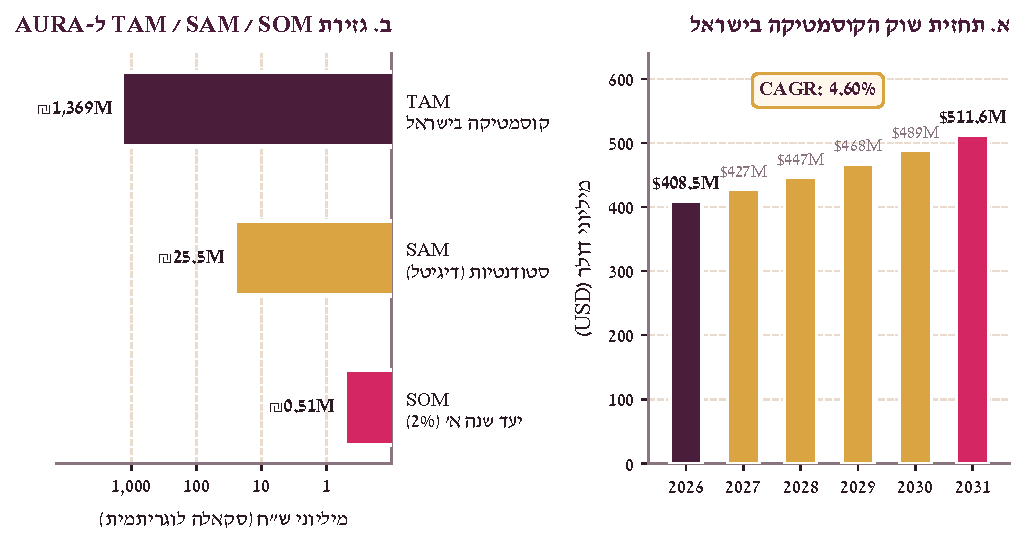
\includegraphics[width=0.95\linewidth]{market_growth_tam_sam_som.pdf}
  \caption{תחזית צמיחת שוק הקוסמטיקה בישראל (\ltr{2026--2031}) וגזירת \en{TAM},
    \en{SAM} ו-\en{SOM} עבור \en{AURA}. מקורות: \en{Mordor Intelligence}~\cite{mordor2026israel},
    מל"ג~\cite{che2026students}, למ"ס~\cite{cbs2024students} ו-\en{DataReportal}~\cite{datareportal2026israel}}
  \label{fig:market-tam-sam-som}
\end{figure}

מן הנתונים באיור~\ref{fig:market-tam-sam-som} עולה כי השוק המקומי צומח בעקביות
(תוספת של למעלה מ-\ltr{\$103} מיליון בחמש שנים), וכי יעד ה-\en{SOM} של \en{AURA}
מהווה פחות מ-\ltr{0.04\%} מכלל השוק --- יעד שמרני דיו להוכחת התאמת מוצר לשוק
(\en{Product-Market Fit}) בחמישה גווני ליבה בלבד.

\begin{insightbox}[בפרויקט שלנו: היתרון המבני של מיקוד בפרסונת ``נור'']
ריכוזן של למעלה מ-\ltr{211} אלף סטודנטיות ב-\ltr{57} קמפוסים אקדמיים, בעלות
חפיפה גבוהה בשימוש ב-\en{TikTok} וב-\en{Instagram}, מאפשר ל-\en{AURA} לשלב
קמפיין תוכן דיגיטלי עם פעילות שטח חווייתית (דוכן טעימות בקמפוס) ולהוריד את עלות
רכישת הלקוחה בהשוואה להשקה ארצית מפוזרת.
\end{insightbox}

\section{ניתוח הנוף התחרותי ומוצרים מתחרים}
\label{sec:market-competitors}

בדיקת שטח דיגיטלית מאומתת (נובמבר \ltr{2026}) מול אתרי המותגים הרשמיים ואתרי
מכירה הפעילים בישראל חשפה קיטוב חד ומפתיע בשוק טינט השפתיים המקומי. בניגוד
להערכות ראשוניות, ארבעה מתוך חמשת המותגים המוכרים ביותר סובלים מפערי מחיר או
זמינות מובהקים בישראל: \en{Rhode} (\ltr{\$20} ל-\ltr{10} מ"ל בארה"ב)
ו-\en{Rare Beauty} (\ltr{\$24} ל-\ltr{3.0} מ"ל בלבד) אינן שולחות ישירות לישראל,
ולכן מחירן אצל משווקי יבוא מקביל מקומיים מזנק ל-\ltr{155--175} ש"ח
ול-\ltr{110--140} ש"ח בהתאמה~\cite{rhode2026tint,rhode2026terms,makeupstore2026rhode,rarebeauty2026lipoil,makeupstore2026rare}.
\en{Benefit Benetint} (\ltr{\$28} ל-\ltr{6} מ"ל בארה"ב) אינו משווק באופן שוטף
בסופר-פארם או ב-\en{BE}, ונרכש בעיקר בדיוטי פרי או באתרי חו"ל בטווח
\ltr{99--125} ש"ח~\cite{benefit2026benetint,caretobeauty2026benefit}.
\en{Fenty Beauty Poutsicle} (\ltr{\$28}) אמנם שולח ישירות לישראל, אך דמי משלוח
ומסים מעלים את מחירו לכ-\ltr{130--160} ש"ח~\cite{fenty2026poutsicle,fenty2026shipping}.
מנגד, \en{Essence} זמין מיידית בסופר-פארם סביב \ltr{15} ש"ח ל-\en{What a Tint!}
(\ltr{4.9} מ"ל) ו-\ltr{6--10} ש"ח ל-\en{Juicy Bomb}~\cite{essence2026superpharm},
אך ללא ערך מותגי או נרטיב חושי. טבלה~\ref{tab:competitors} מרכזת את ההשוואה המלאה.

\begin{table}[htb]
  \caption{השוואת מתחרים מאומתת בקטגוריית טינט ושמן השפתיים בישראל (נובמבר \ltr{2026})}
  \label{tab:competitors}
  \centering\auratablestripes
  \setlength{\tabcolsep}{4pt}
  \scriptsize
  \begin{tabular}{>{\raggedleft\arraybackslash}p{2.15cm} >{\raggedleft\arraybackslash}p{2.05cm} >{\raggedleft\arraybackslash}p{1.65cm} >{\raggedleft\arraybackslash}p{1.65cm} >{\raggedleft\arraybackslash}p{2.45cm} >{\raggedleft\arraybackslash}p{3.65cm}}
    \headrow \hcell{מותג ומוצר} & \hcell{מחיר בישראל (ובארה"ב)} & \hcell{נפח ועלות למ"ל} & \hcell{מגוון גוונים} & \hcell{ערוצי מכירה וזמינות בישראל} & \hcell{מיצוב ובידול \en{AURA} מולו} \\
    \en{Rhode (Peptide Lip Tint)}~\cite{rhode2026tint,rhode2026terms,makeupstore2026rhode} &
      \ltr{155--175} ש"ח (\ltr{\$20}) &
      \ltr{10} מ"ל (\ltr{16.5} ש"ח/מ"ל) &
      \ltr{6--8} גוונים ועונתיים &
      אין משלוח ישיר; יבוא מקביל ומשלחים בלבד &
      יוקרה קרה (\en{Clean Girl}); \en{AURA} מציעה חמימות, זמינות מקומית ומחיר נגיש פי \ltr{2.4} \\
    \en{Benefit (Benetint)}~\cite{benefit2026benetint,caretobeauty2026benefit} &
      \ltr{99--125} ש"ח (\ltr{\$28} ל-\ltr{6} מ"ל) &
      \ltr{6} מ"ל (\ltr{18.7} ש"ח/מ"ל) &
      \ltr{3} גוונים (ורד, פטל, דובדבן) &
      דיוטי פרי ואתרי חו"ל; לא בסופר-פארם &
      מוצר איקוני במרקם מימי; \en{AURA} מציעה פורמולה קרמית-מלחחת ושפה עכשווית \\
    \en{Rare Beauty (Soft Pinch Oil)}~\cite{rarebeauty2026lipoil,makeupstore2026rare} &
      \ltr{110--140} ש"ח (\ltr{\$24}) &
      \ltr{3.0} מ"ל (\ltr{41.7} ש"ח/מ"ל) &
      \ltr{8} גוונים טבעיים וורודים &
      אין משלוח ישיר; בוטיקים ויבוא מקביל &
      אג'נדה רגשית-ערכית; \en{AURA} מתמקדת בעונג קולינרי ובנפח גדול פי \ltr{3.3} \\
    \en{Fenty Beauty (Poutsicle)}~\cite{fenty2026poutsicle,fenty2026shipping} &
      \ltr{130--160} ש"ח (\ltr{\$28} + משלוח) &
      \ltr{3} גר' ($\sim$\ltr{6.5} מ"ל) &
      \ltr{4--6} גוונים עזים וטרופיים &
      משלוח ישיר מהאתר עם דמי משלוח ומסים &
      נועז ועשיר בפיגמנט; \en{AURA} מותאמת למראה טבעי יומיומי לקמפוס במחיר סטודנטיאלי \\
    \en{Essence (What a Tint!)}~\cite{essence2026superpharm} &
      \ltr{15} ש"ח (גלוס \ltr{6--10}) &
      \ltr{4.9} מ"ל (\ltr{3.1} ש"ח/מ"ל) &
      \ltr{1--2} גוונים בסיסיים &
      זמינות מיידית בסופר-פארם וברשתות פארם &
      מוצר דיסקאונט פונקציונלי; \en{AURA} בונה אביזר \en{Masstige} שנור גאה לצלם \\
    \textbf{\en{AURA} (יעד השקה)} &
      \textbf{\ltr{69} ש"ח (מארז \ltr{5}: \ltr{299})} &
      \textbf{\ltr{10} מ"ל (\ltr{6.9} ש"ח/מ"ל)} &
      \textbf{\ltr{5} גווני מזון טבעיים} &
      \textbf{אתר \en{D2C} ישראלי + דוכני טעימות בקמפוס} &
      \textbf{חלל הזדמנות \en{Masstige}:} שיווק חושי חם בהשראת מזון, לחות וזמינות מקומית \\
    \bottomrule
  \end{tabular}
\end{table}

בחינת טבלה~\ref{tab:competitors} חושפת שלוש קבוצות תחרות שכל אחת מהן מותירה
פער צרכני מובהק: (א) \textbf{מותגי הפרימיום הוויראליים מיבוא} (\en{Rhode},
\en{Rare Beauty}, \en{Fenty Beauty}) יוצרים נחשקות גבוהה אך מטילים על סטודנטית
ישראלית עלות של \ltr{110--175} ש"ח (עד \ltr{41.7} ש"ח למיליליטר ב-\en{Rare Beauty})
וחיכוך של משלוחים או יבוא מקביל; (ב) \textbf{מותג המסורת \en{Benefit}} נשען על
נוסטלגיה ומרקם מימי עם \ltr{3} גוונים בלבד וזמינות מדף מוגבלת בארץ; ו-(ג)
\textbf{מותגי הפארם המוזלים (\en{Essence})} פותרים את סוגיית המחיר והזמינות, אך
נעדרים הון חברתי (\en{Social Currency}) ונרטיב קולינרי המניע שיתוף אורגני
ב-\en{TikTok}.

\section{מיצוב מחיר מול ערך וזיהוי חלל ההזדמנות}
\label{sec:market-positioning}

לצורך מפת מיצוב כמותית ושקופה הוגדר \textbf{מדד ערך חושי-מותגי ונגישות} בסולם
\ltr{1--10}, כסכום ארבעה קריטריונים בעלי משקל שווה (\ltr{0--2.5} נקודות לכל אחד):
(א) \textbf{נרטיב קולינרי וטרנדיות} --- עומק השימוש בשמות מאכלים, ניחוחות
ו-\en{Appetite Appeal}; (ב) \textbf{פורמולה היברידית מלחחת} --- שילוב גוון טבעי
עם תחושת לחות קרמית לא מייבשת; (ג) \textbf{אסתטיקת אריזה והון חברתי} --- נחשקות
כ``אביזר תיק'' ופוטנציאל ויראליות (ל-\en{AURA} ניתן ציון שמרני של \ltr{1.8} לעומת
\ltr{2.5} ל-\en{Rhode}, כהכרה ריאלית בהיעדר הילת סלבריטאית בפתיחה); ו-(ד)
\textbf{נגישות מקומית ותמורה לנפח בישראל} --- רכישה ישירה, משלוח מהיר והוגנות
המחיר למיליליטר. טבלה~\ref{tab:value-index} מפרטת את הציונים, ואיור~\ref{fig:price-positioning}
ממפה את המחיר המאומת בישראל מול מדד הערך הכולל.

\begin{table}[htb]
  \caption{פירוט ניקוד מדד הערך החושי-מותגי והנגישות (\ltr{0--2.5} לכל קריטריון, סך הכול עד \ltr{10})}
  \label{tab:value-index}
  \centering\auratablestripes
  \setlength{\tabcolsep}{4pt}
  \footnotesize
  \begin{tabular}{>{\raggedleft\arraybackslash}p{3.6cm} r r r r r}
    \headrow \hcell{מותג ומוצר} & \hcell{נרטיב קולינרי} & \hcell{פורמולה מלחחת} & \hcell{הון חברתי} & \hcell{נגישות בישראל} & \hcell{ציון כולל} \\
    \en{Essence (What a Tint!)} & \ltr{0.5} & \ltr{1.0} & \ltr{0.8} & \ltr{2.5} & \ltr{4.8} \\
    \en{Benefit (Benetint)} & \ltr{0.8} & \ltr{0.8} & \ltr{2.0} & \ltr{1.2} & \ltr{4.8} \\
    \en{Rare Beauty (Soft Pinch)} & \ltr{1.0} & \ltr{2.2} & \ltr{2.3} & \ltr{1.0} & \ltr{6.5} \\
    \en{Fenty Beauty (Poutsicle)} & \ltr{1.2} & \ltr{1.8} & \ltr{2.2} & \ltr{1.4} & \ltr{6.6} \\
    \en{Rhode (Peptide Lip Tint)} & \ltr{2.4} & \ltr{2.4} & \ltr{2.5} & \ltr{0.6} & \ltr{7.9} \\
    \textbf{\en{AURA} (יעד השקה)} & \textbf{\ltr{2.4}} & \textbf{\ltr{2.2}} & \textbf{\ltr{1.8}} & \textbf{\ltr{2.4}} & \textbf{\ltr{8.8}} \\
    \bottomrule
  \end{tabular}
\end{table}

\begin{figure}[htb]
  \centering
  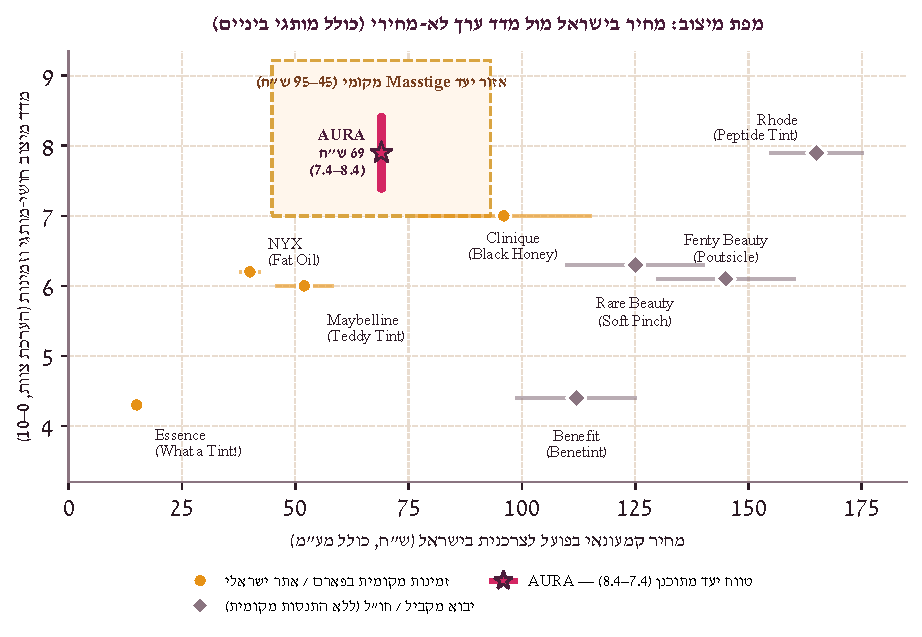
\includegraphics[width=0.86\linewidth]{price_positioning.pdf}
  \caption{מפת מיצוב: מחיר בפועל לצרכנית בישראל (עם טווחי מחיר מאומתים) מול מדד
    הערך החושי-מותגי והנגישות. האזור המוצלל מסמן את חלל ההזדמנות בקטגוריית
    ה-\en{Masstige} המקומית (\ltr{45--95} ש"ח)}
  \label{fig:price-positioning}
\end{figure}

מפת המיצוב באיור~\ref{fig:price-positioning} מציגה בבירור את ההזדמנות העסקית:
בין פלח הפארם המוזל (\ltr{10--20} ש"ח) לבין אשכול הפרימיום המיובא
(\ltr{99--175} ש"ח) פעור \textbf{חלל הזדמנות (\en{White Space}) רחב בטווח
\ltr{45--95} ש"ח}. תמחור היעד של \en{AURA} ב-\ltr{69} ש"ח ל-\ltr{10} מ"ל
(\ltr{6.9} ש"ח/מ"ל) זול בכ-\ltr{58\%} ממחיר \en{Rhode} בישראל ובכ-\ltr{45\%}
מ-\en{Rare Beauty}, ועדיין שומר על פער מיצובי ברור מעל מוצרי הפארם הזולים ---
פער חיוני לבניית דימוי \en{Masstige} איכותי ולמימון חוויית מותג עשירה. בנוסף,
העובדה שכל ארבעת מותגי הפרימיום במפה נרכשים בישראל מרחוק (מעוינים) מונעת מן
הצרכנית להתנסות בניחוח, במרקם ובגוון טרם הקנייה. ממצא זה מוביל ישירות אל
פרק~\ref{ch:alternatives}, שבו יושוו חלופות ההשקה לפי יכולתן לגשר על חסם
ההתנסות החושית תוך שמירה על יתרון המחיר המקומי.

\begin{keymessage}[המסר המרכזי מחקר השוק]
שוק הקוסמטיקה בישראל (\ltr{\$408.5} מיליון ב-\ltr{2026}, צמיחה שנתית של
\ltr{4.60\%}) וזינוק של \ltr{19\%} בקטגוריית השפתיים היוקרתית מייצרים תנאי פתיחה
נוחים ל-\en{AURA}. פערי המחיר והמשלוח של המתחרים הבינלאומיים (\ltr{99--175} ש"ח
בישראל) מותירים חלל \en{Masstige} בלתי תפוס סביב \ltr{69} ש"ח --- חלל שבו ניתן
להשיג יעד ריאלי של כ-\ltr{2\%} משוק הסטודנטיות הפעילות בשנה הראשונה (כ-\ltr{511}
אלף ש"ח) באמצעות שילוב של חמימות קולינרית, לחות וזמינות מקומית מיידית.
\end{keymessage}

% =====================================================================
%  Chapter 5: Design alternatives                 Page budget: 8 (pp. 23-30)
%  Booklet: alternatives, weighted decision matrix (weights sum to 1.0),
%           chosen architecture, innovation.
%  Owner: Raghad (Antigravity) - only she edits this file
% =====================================================================
\chapter{חלופות לתוכנית ההשקה}
\label{ch:alternatives}

\section{החלופות}
\draftnote{שלוש חלופות השקה לפחות (למשל: חנות מקוונת בלבד, קמעונאות, שיתוף פעולה עם משפיעניות).}

\section{מטריצת החלטה משוקללת}
\draftnote{קריטריונים, משקלים שסכומם \ltr{1.0}, ציון לכל חלופה ונוסחת הציון המשוקלל.}

\section{החלופה הנבחרת}
\draftnote{תרשים \en{TikZ} של מבנה ההשקה שנבחר: ערוצים, שלבים ותוצרים.}

\section{החדשנות}
\draftnote{מה חדש ב-\en{AURA} לעומת מה שקיים בשוק.}

% =====================================================================
%  Chapter 6: Work plan                           Page budget: 4 (pp. 31-34)
%  Booklet: WBS, RACI, Gantt chart, milestones, critical path.
%  Owner: Raghad (Antigravity) - only she edits this file
% =====================================================================
\chapter{תוכנית עבודה}
\label{ch:workplan}

\section{מבנה פירוק העבודה}
\draftnote{\en{WBS}: חבילות עבודה ותוצר לכל חבילה.}

\section{חלוקת אחריות}
\draftnote{מטריצת \en{RACI}.}

\section{לוח זמנים ואבני דרך}
\draftnote{תרשים גאנט, נתיב קריטי ואבני דרך.}

% =====================================================================
%  Chapter 7: Risk management                     Page budget: 2 (pp. 35-36)
%  Booklet: failure modes, probability x impact (R = P x I),
%           risk matrix, mitigation + contingency for every R >= 12.
%  Owner: Raghad (Antigravity) - only she edits this file
% =====================================================================
\chapter{ניהול סיכונים}
\label{ch:risks}

\section{זיהוי והערכת סיכונים}
\draftnote{טבלת סיכונים עם הסתברות \en{P}, השפעה \en{I} וציון $R = P \times I$, ומטריצת סיכונים.}

\section{תוכנית הפחתה}
\draftnote{לכל סיכון עם $R \geq 12$: פעולת מנע, תוכנית מגירה וסיכון שיורי.}

% =====================================================================
%  Chapter 8: Summary                             Page budget: 1 (p. 37)
%  Booklet: findings, design readiness, immediate next steps.
%  Owner: Raneem (Claude Code) - only she edits this file
% =====================================================================
\chapter{סיכום}
\label{ch:summary}

\draftnote{הממצאים העיקריים, מוכנות לביצוע, והצעדים המיידיים הבאים.}

\begin{keymessage}
המסר המרכזי למנהלים, במשפט אחד או שניים, ייכתב כאן.
\end{keymessage}


% ----- References -----
\printreferences

\end{document}
